%% Technische Begutachtung
% Aufgabe 2
\section{Technische Begutachtung}

\subsection{Referenz-Steuerungskennlinie}

Für die Erstellung der Referenz-Steuerungskennlinie kommt die Software \texttt{QBlade v.0.99c} zum Einsatz. Bei dem zugrundeliegendenden Modell handelt es sich um eine \SI{10}{\mw} Referenzanlage der \gls{IEA}.\medskip

Nachdem das Modell mit \texttt{QBlade} geöffnet wurde, muss das Fenster für die Simulation der Anlage nach der \gls{BEM} Methode geöffnet werden. Vorteil der \gls{BEM} Methode ist in erster Linie die geringe Berechnungszeit und somit eine schnelle Entwicklung von Rotorblättern und der Vergleich dieser untereinander. In dem nun geöffneten Fenster wird die \glqq Char \gls{BEM}\grqq{} ausgewählt. In diesem können anschließend die Parameter für die Simulation eingestellt werden.

\begin{figure}[H]
    \centering
    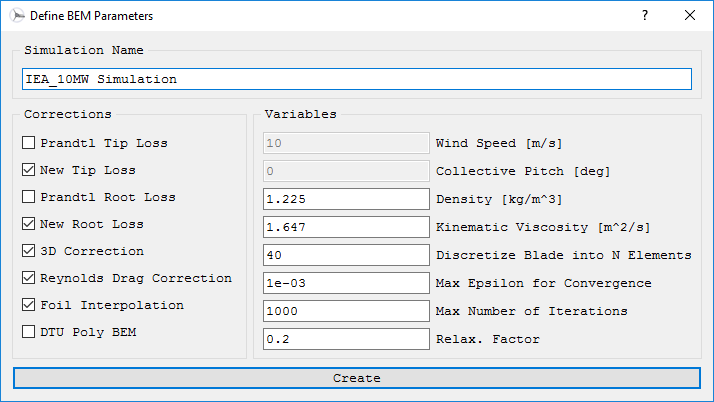
\includegraphics[width=\textwidth]{Bilder/QBlade_CharBEM_SimParas}
    \caption{Verwendete Parameter für die BEM Simulation}\label{fig:SimParas}
\end{figure}

In \autoref{fig:SimParas} sind die verwendeten Simulationsparameter dargestellt. Hier können verschiedene Korrekturen für z.B. Blattspitzen und -füße eingestellt werden. Weiterhin können die physikalischen Variablen und Simulationsparameter eingestellt werden, um die Simulation dem respektivem Standort anzupassen.

\begin{itemize}
	\item Luftdichte
	\item Die kinematische Viskosität der Luft
	\item Anzahl der Blattelemente
	\item Den $\epsilon$ des Grenzwerts der Iteration
	\item Die maximale Anzahl der Iterationsschritte
	\item Den Entspannungsfaktor $\omega_{\text{relax}}$ der Grenzwertberechnung
\end{itemize}

Anschließend müssen noch die gewünschten Parameter (Minimum, Maximum und Schrittweite) für die Parametervariation der Simulation eingestellt werden. Hierzu zählen folgende Parameter:

\begin{itemize}
	\item Windgeschwindigkeit
	\item Die Drehzahl der \gls{WKA}
	\item Den Pitchwinkel der \gls{WKA}
\end{itemize}

\begin{figure}[H]
    \centering
    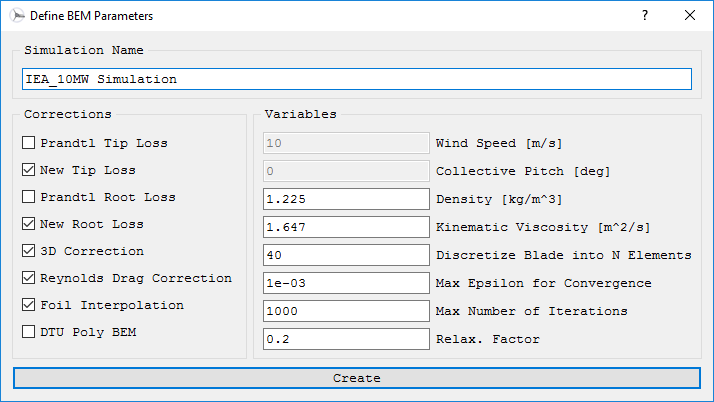
\includegraphics[width=\textwidth]{Bilder/QBlade_CharBEM_SimParas}
    \caption{Verwendete Parametervariation der BEM Char Simulation}\label{fig:SimParas2}
\end{figure}

Die verwendeten Parameter finden sich in \autoref{fig:SimParas2}. Um den gewünschten Export der Daten vornehmen zu können, muss in einem der verfügbaren Felder für graphische Darstellungen der $c_\text{p}$ über den \gls{TSR} dargestellt werden. Anschließend müssen per Rechtsklick noch die Kurvenschar im Abhängigkeit von der Drehzahl und dem Pitchwinkel dargestellt werden. Die entsprechenden Einstellungen finden sich in \autoref{fig:GraphParas}.

\begin{figure}[H]
    \centering
    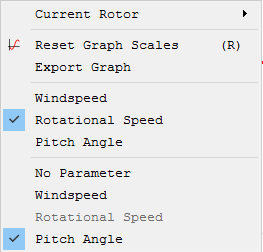
\includegraphics[width=0.6\textwidth]{Bilder/QBlade_CharBEM_GraphParas}
    \caption{Einstellungen für die Darstellung des $c_\text{p}$-$\lambda$-Kennfelds}\label{fig:GraphParas}
\end{figure}

Durch einen weiteren Rechtsklick auf die Kurvenschar, können die zugrundeliegenden Daten exportiert werden. Hierbei wird der Export als \texttt{CSV} gewählt. Anschließend müssen in den Daten noch die überflüssigen Datenreihen des \gls{TSR} entfernt werden. Hierbei handelt es sich um Duplikate Abschließend werden die Schritte der Anleitung von \texttt{moodle} durchgeführt.\medskip

Für die Erstellung der $P$-$\omega$-Kennlinie wird nun eine weitere Simulation im \glqq Turbine \gls{BEM}\grqq{} Fenster durchgeführt. In diesem Fall kann für Parametervariation die Windgeschwindigkeit eingestellt werden. In \autoref{fig:SimParasTurbine} finden sich die verwendeten Parameter.

\begin{figure}[H]
    \centering
    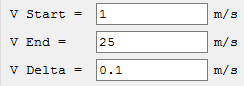
\includegraphics[width=0.6\textwidth]{Bilder/QBlade_TurbineBEM_SimParas}
    \caption{Verwendete Parametervariation der BEM Turbine Simulation}\label{fig:SimParasTurbine}
\end{figure}

Nach Abschluss der Simulation wird in einem Graphen die Leistung $P$ über die Winkelgeschwindigkeit $\omega$ dargestellt und per Rechtsklick die Option \glqq Set as Rotor Graph\grqq{} eingestellt. Die zugrundeliegenden Daten werden abschließend ebenfalls per Rechtsklick exportiert und nach der Anleitung in das \texttt{Simulink} Modell integriert.

\subsection{Simulationen Netzfehler als Plausibilitätsprüfung}

\subsection{Anforderungen der VDE AR-4110 {--} Anschluss am Mittelspannungsnetz}

\subsection{Untersuchung Inselnetz}